\newpage
\section{Resultados}

\subsection{Circuito de proteção com diodo Zener}

Através da variação da quantidade de massa sobre o \textit{Strain Gauge} montado no circuito da figura \ref{f_sch}, foi possível gerar a seguinte tabela de medidas.

\begin{small}
    \begin{table}[H]
        \begin{center}
            \caption{Tensão de entrada e tensão de saída para o diodo zener.}
            \begin{tabular}{l|l|l|l}
                \hline
                \multirow{2}{50pt}{Número de peças } & $V_{out1}$ & $V_{out2}$ & $V_{out3}$ \\
                & & & \\
                \hline
                1 & 0.08 & 0.06 & 0.03 \\
                2 & 0.49 & 0.48 & 0.56 \\
                3 & 1.01 & 1.09 & 1.12 \\
                4 & 1.49 & 1.62 & 1.71 \\
                5 & 2.01 & 2.10 & 2.28 \\
                6 & 2.39 & 2.86 & 2.95 \\
                7 & 3.33 & 3.49 & 3.49 \\
                8 & 3.42 & 3.78 & 3.54 \\
                9 & 3.77 & 3.83 & 3.98 \\
                10 & 5.12 & 5.29 & 5.37 \\
                11 & 5.13 & 5.17 & 5.18 \\ 
                \hline
            \end{tabular}
            \label{t_zener}
        \end{center}
    \end{table}
\end{small}

Através dos valores da tabela, foi gerado um gráfico com o auxílio do software MATLAB para melhor visualização dos resultados.

\begin{figure}[H]
    \centering
    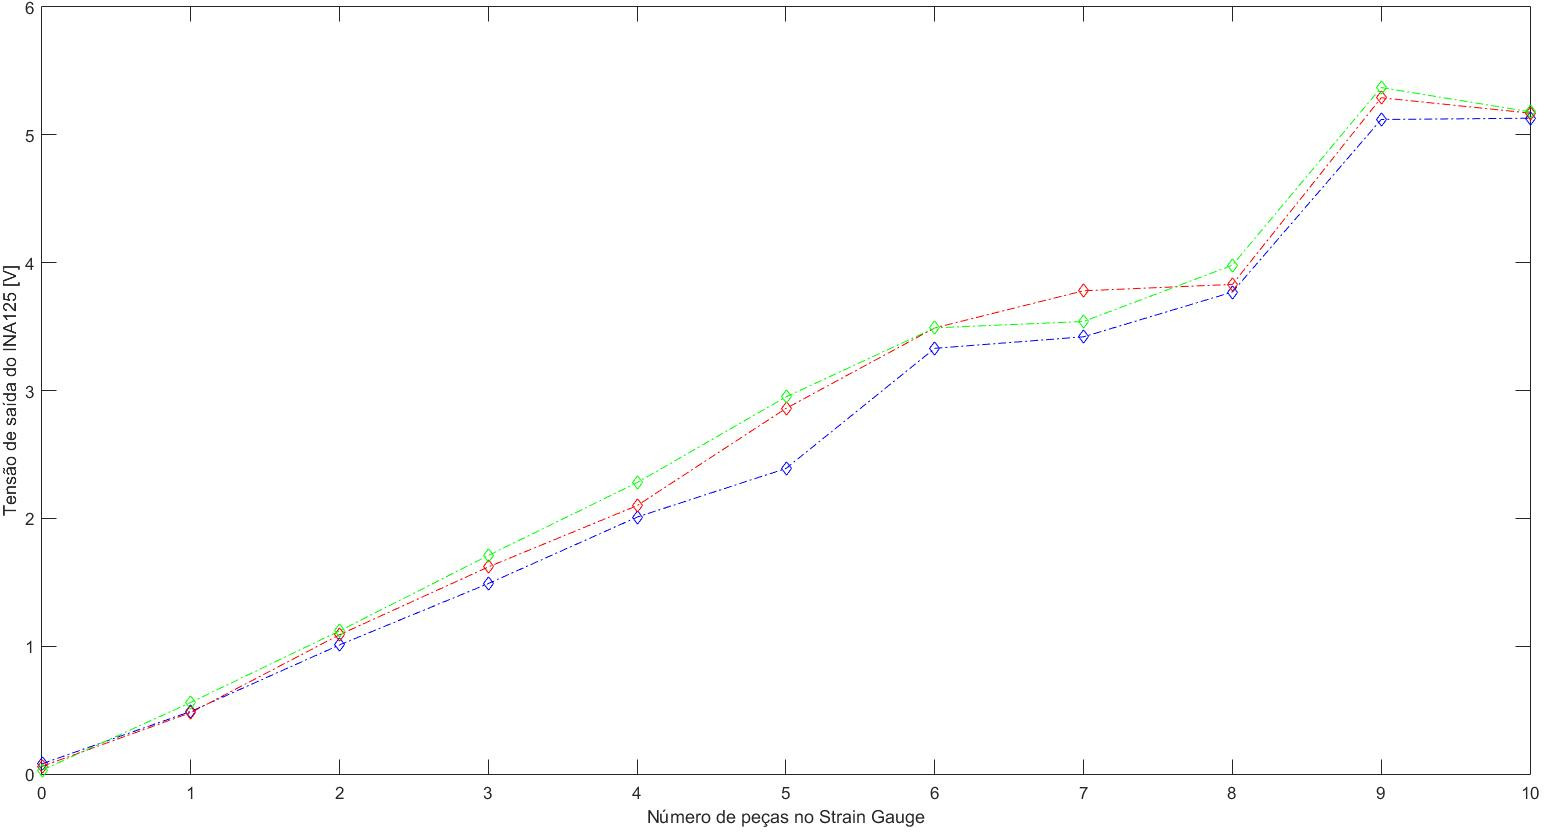
\includegraphics[scale=0.3]{img/data.jpg}
    \caption{Gráfico da saída em tensão ($V_{out}$) em função do número de peças.}
    \label{f_plottermistor}
\end{figure}

Pode-se observar nas 3 curvas das medidas obtidas, uma leve variação nos parâmetros devido à incerteza.

